\lecture{1}{Фундамент}

\section{Фундамент}
\subsection{1 Вопрос}
\subsubsection{Компилируемость/интерпретируемость}
\begin{definition}{Компилируемость(из википедии)}{}
\textbf{Компилируемый язык программирования} — язык программирования, исходный код которого преобразуется компилятором в машинный код и записывается в файл с особым заголовком и/или расширением для последующей идентификации этого файла, как исполняемого операционной системой.
\end{definition}
\begin{definition}{Интерпретируемость}{}
\textbf{Интерпретируемый язык программирования} — язык программирования, исходный код которого выполняется интерпретатором, он берет оператор, транслирует его в машинный код, и выполняет его.
\end{definition}
\textbf{Сравнение}
\begin{itemize}
    \item Компилируемые языки обычно быстрее
    \item Интерпретируемые языки более гибкие
    \item Компилируемые языки требуют более долгой сборки
    \item Дебаг интерпертируемых проще
\end{itemize}
\subsubsection{Заголовочные файлы и их подключение}
\begin{definition}{Заголовочный файл}{}
  \textbf{Заголовочный файл в С++} --- файлы с классами и т.п. . Они подставляются в прекомпайле, просто ctrl+c ctrl+v в основной файл с помощью \texttt{\#include}. Для подстановки либ и системных файлов используют \verb|<>|, а для тех который навайбкодил сам --- \verb|""|.
\end{definition}
Директивы в исходном файле сообщают препроцессору о выполнении определенных действий
\begin{implementation}{Пример подключения заголовочного файла}{}
\begin{lstlisting}[language=c++]
#include <iostream>
#include "myheader.h"
\end{lstlisting}
\end{implementation}
\subsubsection{Переменные: объявление, использование, хранение}
\begin{definition}{Переменная}{}
\textbf{Переменная} --- по сути, просто кусок памяти, зарезервированный для использования программой. Вы обращаетесь к ней, используя имя переменной. Типы в  C++ определяют размер блока памяти и как читать эту память.Чтобы создать переменную в C++, вам нужны как минимум две вещи: \textbf{имя и тип}.
\end{definition}
\begin{definition}{идентификаторы}{}
  \textbf{Имена переменных} — это идентификаторы(там еще классы, функции, пространства имен). Могут содержать символы a-z, A-Z, 0-9 и \_, не начинаться с цифры или \_, и не быть ключевым словом. Есть и другие правила.
\end{definition}
\begin{definition}{Type}{}
  C++ — строго типизированный язык.
\end{definition}
\begin{implementation}{Использование переменных}{}
\begin{lstlisting}[language=C++]
#include <iostream>

int main() {
    int v1 = 42;
    std::cout << v1 << '\n';
    v1 = 69;
    std::cout << v1 << '\n';
    double temp_in_F = 72;
    double temp_in_C = (temp_in_F - 32) / 1.8;
    std::cout << temp_in_F << "degrees Fahrenheit is " <<
               temp_in_C << "degrees Celsius " << '\n';

    temp_in_F = 95.5;
    temp_in_C = (temp_in_F - 32) / 1.8;
    std::cout << temp_in_F << "degrees Fahrenheit is " <<
               temp_in_C << "degrees Celsius " << '\n';

    return 0;
}
\end{lstlisting}
\end{implementation}
\subsubsection*{auto}
Подробнее в \ref{auto}
\subsubsection{Работа с потоком ввода/вывода}
\begin{definition}{Поток ввода/вывода}{}
  Это стандартные потоки(смотри конспект по тулзам(там когда то давно я писал его, ну халява лютая)), такие как STDIN, STDOUT и STDERR. Для них есть iostream, в ней есть \texttt{std::cin}, \texttt{std::cout} и \texttt{std::cerr}. У каждого из них есть операторы \texttt{$<<$} и \texttt{$>>$}
\end{definition}
Виды манипуляторов с выводом:
\begin{itemize}
  \item \texttt{std::endl} --- перевод строки и сброс буфера
  \item \texttt{std::flush} --- сброс буфера
  \item \texttt{std::setw(n)} --- установка ширины поля вывода
  \item \texttt{std::setprecision(n)} --- установка точности вывода для чисел с плавающей точкой
  \item \texttt{std::fixed} --- вывод чисел с плавающей точкой в фиксированном формате
  \item \texttt{std::scientific} --- вывод чисел с плавающей точкой в научном формате
  \item \texttt{std::hex}, \texttt{std::dec}, \texttt{std::oct} --- установка системы счисления для вывода целых чисел
  \item \texttt{std::boolalpha}, \texttt{std::noboolalpha} --- вывод булевых значений как \texttt{true}/\texttt{false} или \texttt{1}/\texttt{0}
\end{itemize}
\subsubsection{Статическая/динамическая типизация}
\begin{definition}{Статическая типизация}{}
\textbf{Статическая типизация} --- переменная, параметр подпрограммы, возвращаемое значение функции связывается с типом в момент объявления и живет с ним до конца.
\end{definition}
\begin{definition}{Динамическая типизация}{}
\textbf{Динамическая типизация} --- переменная связывается с типом в момент присваивания значения, а не в момент объявления переменной.
\end{definition}
\textbf{Сильная и слабая типизация}
\textbf{Кратко:} при слабой типизации тип можно например привести один к другому. При сильной нет.
\textbf{Некратко:}
\begin{itemize}
  \item \textbf{Сильная типизация:}
    система типов языка программирования не допускает неявного преобразования одного типа к другому.
    Любое приведение типов должно быть явно указано программистом.
  \item \textbf{Слабая типизация:}
    язык позволяет неявные преобразования между различными типами.
    Тип одной переменной можно, например, автоматически привести к другому типу.
\end{itemize}
\subsubsection{Основные типы и операции над ними}
\textbf{ТИПЫ В С++}
\begin{itemize}
  \item \textbf{Знаковые целые}, может хранить от $-(2^{15} -1)$ до $(2^{15} -1).$ Обычно это \texttt{int}, \texttt{short}, \texttt{long}, \texttt{long long}.
  \item \textbf{Беззнаковые целые}, может хранить от $0$ до $2^{16} -1.$ Обычно это \texttt{unsigned int}, \texttt{unsigned short}, \texttt{unsigned long}, \texttt{unsigned long long}.
  \item \textbf{Символьные типы} хранят буквы, цифры, знаки препинания и управляющие коды. Обычно это \texttt{char}, \texttt{wchar\_t}, \texttt{char16\_t}, \texttt{char32\_t}.
  \item \textbf{Типы с плавающей точкой} хранения вещественных чисел в виде мантиссы и экспоненты; могут хранить очень большие и очень маленькие значения
\end{itemize}
Пример хранения float в памяти:
\usetikzlibrary{chains, decorations.pathreplacing}
\begin{figure}[htp]

\resizebox{\textwidth}{!}{%
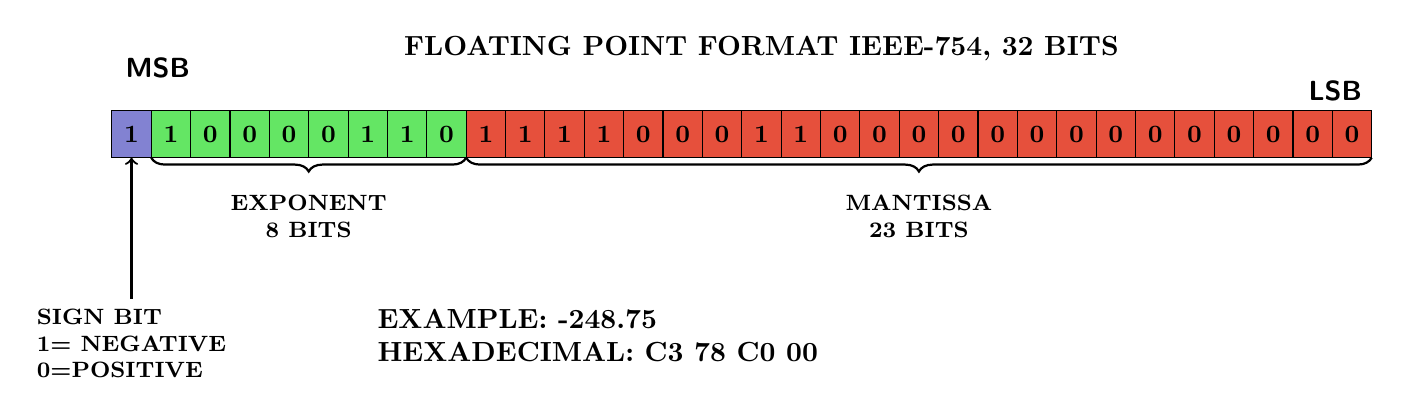
\begin{tikzpicture}[
  font=\sffamily,
  node distance=0cm,
  start chain=chain-1 going right,
  box/.style={
    draw, minimum width=0.5cm, minimum height=0.6cm,
    outer sep=0pt, on chain=chain-1, font=\small\bfseries
  }
]

  % Title
  \node[anchor=south, font=\bfseries] at (8, 0.8) {FLOATING POINT FORMAT IEEE-754, 32 BITS};

  % Colors based on the image (Byte-aligned coloring)
  \definecolor{cSign}{RGB}{130,130,210}   % Dark Blue
  \definecolor{cByte1}{RGB}{180,180,230}  % Light Blue
  \definecolor{cByte2}{RGB}{255,255,100}  % Yellow
  \definecolor{cByte3}{RGB}{230,80,60}    % Red
  \definecolor{cByte4}{RGB}{100,230,100}  % Green

  % MSB Label
  \node[anchor=south west] at (-0.2, 0.6) {\textbf{MSB}};

  % --- BITS (Hex: C3 78 C0 00) ---

  % Byte 1: C3 -> 1 1000011
  \node [box, fill=cSign] (bit31) {1}; % Sign bit
  \node [box, fill=cByte4] {1};
  \node [box, fill=cByte4] {0};
  \node [box, fill=cByte4] {0};
  \node [box, fill=cByte4] {0};
  \node [box, fill=cByte4] {0};
  \node [box, fill=cByte4] {1};
  \node [box, fill=cByte4] {1};

  % Byte 2: 78 -> 01111000
  \node [box, fill=cByte4] {0};
  \node [box, fill=cByte3] {1};
  \node [box, fill=cByte3] {1};
  \node [box, fill=cByte3] {1};
  \node [box, fill=cByte3] {1};
  \node [box, fill=cByte3] {0};
  \node [box, fill=cByte3] {0};
  \node [box, fill=cByte3] {0};

  % Byte 3: C0 -> 11000000
  \node [box, fill=cByte3] {1};
  \node [box, fill=cByte3] {1};
  \node [box, fill=cByte3] {0};
  \node [box, fill=cByte3] {0};
  \node [box, fill=cByte3] {0};
  \node [box, fill=cByte3] {0};
  \node [box, fill=cByte3] {0};
  \node [box, fill=cByte3] {0};

  % Byte 4: 00 -> 00000000
  \node [box, fill=cByte3] {0};
  \node [box, fill=cByte3] {0};
  \node [box, fill=cByte3] {0};
  \node [box, fill=cByte3] {0};
  \node [box, fill=cByte3] {0};
  \node [box, fill=cByte3] {0};
  \node [box, fill=cByte3] {0};
  \node [box, fill=cByte3] {0};

  % LSB Label
  \node[anchor=south east] at (chain-1-32.north east) {\textbf{LSB}};

  % --- BRACES ---
  % Exponent: Bits 30-23 (Indices 2 to 9 in chain)
  \draw[decorate, decoration={brace, amplitude=5pt, mirror}, thick]
    (chain-1-2.south west) -- (chain-1-9.south east)
    node[midway, below=10pt, align=center, font=\bfseries\footnotesize] {EXPONENT\\8 BITS};

  % Mantissa: Bits 22-0 (Indices 10 to 32 in chain)
  \draw[decorate, decoration={brace, amplitude=5pt, mirror}, thick]
    (chain-1-10.south west) -- (chain-1-32.south east)
    node[midway, below=10pt, align=center, font=\bfseries\footnotesize] {MANTISSA\\23 BITS};

  % --- ANNOTATIONS ---
  % Sign Bit Arrow
  \draw[<-, thick] (bit31.south) -- ++(0,-1.8)
    node[below, align=left, font=\bfseries\footnotesize, anchor=north] (signtext) {SIGN BIT\\1= NEGATIVE\\0=POSITIVE};

  % Example Text
  \node[right=3cm of signtext.north, anchor=north west, align=left, font=\bfseries] {
    EXAMPLE: -248.75\\
    HEXADECIMAL: C3 78 C0 00
  };

\end{tikzpicture}
}
\end{figure}
\textbf{ОПЕРАЦИИ НАД ТИПАМИ}
\begin{itemize}
  \item арифметические операции +, -, *, /, \, \%
  \item побитовые операции \texttt{\&}, \texttt{|}, \texttt{\^{}}, \texttt{<<}, \texttt{>>}
  \item логические операции \texttt{\&\&}, \texttt{||}
\end{itemize}
\subsubsection{Литералы и идентификаторы}
\begin{definition}{Примеры литералов}{}
\begin{itemize}
  \item \texttt{5} --- целочисленный литерал (\texttt{int})
  \item \texttt{5.0} --- литерал с плавающей точкой двойной точности (\texttt{double})
  \item \texttt{5.0f} --- литерал с плавающей точкой (\texttt{float})
  \item \texttt{'a'} --- символьный литерал (\texttt{char})
  \item \texttt{"aaa"} --- строковый литерал (\texttt{const char*})
  \item \texttt{true} --- булевый литерал (\texttt{bool}), является ключевым словом
\end{itemize}
\end{definition}

\begin{definition}{Примеры идентификаторов}{}
\begin{itemize}
  \item \texttt{x}
  \item \texttt{CoOlFuNcTiOnNaMe}
  \item \texttt{} --- эмоджи. \textit{Примечание: поддерживаются далеко не всеми компиляторами хотя вроде в стандарте говорят что можно, но в латехе не можно, поэтому сами как нибудь}
\end{itemize}
\end{definition}
\subsubsection{Объявления и определения}
\begin{definition}{Объявление}{}
\textbf{Объявление} ---  введение какой-то новой сущности
\end{definition}
\begin{implementation}
{Пример объявления}{}
\begin{lstlisting}[language=C++]
  int a;
  int b = 10;
\end{lstlisting}
\end{implementation}
\begin{definition}
{Определение}{}
\textbf{Определение} --- выделение памяти для сущности
\end{definition}
\begin{implementation}
{Пример определения}{}
\begin{lstlisting}[language=C++]
  int a;
  int b = 10;

  double f(int a);

  int main() {
    f(1);
  }
\end{lstlisting}
Такой код не скомпилируется, потому что f объявили, но не определили ее.
\end{implementation}
\textbf{Замечание:} Каждое определение является объявлением
\subsubsection{скоупы видимости}

\begin{itemize}
  \item \textbf{Глобальная область видимости}: переменные, объявленные вне функций и классов, доступны во всей программе, начиная с точки объявления.
  \item \textbf{Локальная область видимости}: переменные, объявленные внутри функций или блоков кода \verb|{}|, доступны только в рамках этого блока.
  \item \textbf{Вложенные области видимости}: внутри одной области могут быть созданы другие области с помощью блоков \verb|{}|. Внутри вложенной области можно объявлять переменные с теми же именами, что и во внешней.
  \item \textbf{Глобальный доступ}: к переменным глобальной области видимости изнутри функций можно обратиться с помощью оператора \verb|::|.
  \item \textbf{Namespace (пространства имён)}: используется для разделения областей видимости между разными логическими частями кода.
  \item \textbf{Использование namespace}:
    \begin{itemize}
        \item создать и назвать: \verb|namespace N { int x = 10; }|
        \item использовать: \verb|N::x|
        \item достать что то оттуда: \verb|using N::x;|
        \item вложить это пространство имён в наше пространство: \verb|using namespace std;|
    \end{itemize}
\end{itemize}

\begin{lstlisting}[language=C++]
int x = 10;
int main() {
    int x = 5;
    {
        int x = 3;
        std::cout << ::x;
    }
}
\end{lstlisting}

\subsubsection{Выражения и операторы}

\textbf{Выражение}~--- комбинация идентификаторов, литералов и операторов, которая вычисляется в программе.

\begin{itemize}
  \item Примеры выражений:
    \begin{itemize}
      \item \verb|a + 5|
      \item \verb|(--a * b << 3) + 1|
    \end{itemize}
\end{itemize}

\textbf{Операторы}
\begin{itemize}
  \item \textbf{Арифметические:} \verb|+, -, *, /, %|, унарный \verb|+|, унарный \verb|-|
  \item \textbf{Побитовые:} \verb!&, |, ^! (XOR), \verb!~! (побитовое НЕ), \verb!<<, >>!
  \item \textbf{Сравнения:} \verb|==, !=, <, >, <=, >=, <=>| (C++20 spaceship operator)
  \item \textbf{Логические:} \verb+&&, ||, !+
\end{itemize}

\textbf{Примечания:}
\begin{itemize}
  \item Операторы могут вести себя по-разному в зависимости от типа аргументов: например, \verb|<<| для чисел~--- это побитовый сдвиг, а для \verb|std::cout|~--- вывод в поток.
  \item Логические операторы \verb|&&| и \verb||| реализуют \textit{ленивые вычисления}~--- выражение справа вычисляется только если нужно.
  \item \textbf{Инкремент и декремент:} \verb|++| и \verb|--|. Префиксный и постфиксный варианты отличаются тем, что (\verb|++x|) сначала увеличивает значение, а (\verb|x++|)~--- сначала возвращает старое, а затем увеличивает.
\end{itemize}

\begin{lstlisting}[language=C++]
int main() {
    int x = 10;
    std::cout << ++x;   // 11
    std::cout << x;     // 11

    int y = 10;
    std::cout << y++;   // 10
    std::cout << y;     // 11
}
\end{lstlisting}

\subsubsection{Ленивые вычисления}
\begin{definition}
{Ленивые вычисления}{}
Логические операторы \texttt{\&\&} и \texttt{||} не вычисляют лишнего.
Так чтобы вектор удобно проверять, типо есть \texttt{!vec.empty() \&\& vec[0] == 42} и не бояться \texttt{vec[0]} при пустом векторе.
\end{definition}
\subsubsection{Тернарный оператор}
\begin{definition}{Тернарный оператор}{}
Тернарный оператор \texttt{?:} единственный оператор на 3ех аргументах. \newline
формат: \texttt{condition ? expr1 : expr2}
Если \texttt{condition} истинно, то возвращается значение \texttt{expr1}, иначе \texttt{expr2}.
\end{definition}
\subsubsection{Приоритет вызова операторов}
\begin{center}
\begin{tabular}{|c|l|l|c|}
\hline
\textbf{Приоритет} & \textbf{Оператор} & \textbf{Описание} & \textbf{Ассоциативность} \\
\hline
1 & \texttt{::} & Разрешение области видимости & Слева направо \\
\hline
2 & \texttt{++ --} & Постфиксный инкремент/декремент & Слева направо \\
  & \texttt{()} & Вызов функции & \\
  & \texttt{[]} & Индекс массива & \\
  & \texttt{.} \texttt{->} & Доступ к члену & \\
\hline
3 & \texttt{++ --} & Префиксный инкремент/декремент & \textbf{Справа налево} \\
  & \texttt{+ -} & Унарный плюс/минус & \\
  & \texttt{! \~} & Логическое/Побитовое НЕ & \\
  & \texttt{(type)} & Приведение типа (C-style) & \\
  & \texttt{* \&} & Разыменование / Взятие адреса & \\
  & \texttt{sizeof} & Размер типа & \\
  & \texttt{new delete} & Выделение/освобождение памяти & \\
\hline
4 & \texttt{.* ->*} & Доступ к члену по указателю & Слева направо \\
\hline
5 & \texttt{* / \%} & Умножение, деление, остаток & Слева направо \\
\hline
6 & \texttt{+ -} & Сложение, вычитание & Слева направо \\
\hline
7 & \texttt{<< >>} & Побитовый сдвиг & Слева направо \\
\hline
8 & \texttt{<=>} & Трехстороннее сравнение (C++20) & Слева направо \\
\hline
9 & \texttt{< <= > >=} & Операторы сравнения & Слева направо \\
\hline
10 & \texttt{== !=} & Равенство / Неравенство & Слева направо \\
\hline
11 & \texttt{\&} & Побитовое И & Слева направо \\
\hline
12 & \texttt{\^} & Побитовое Исключающее ИЛИ (XOR) & Слева направо \\
\hline
13 & \texttt{|} & Побитовое ИЛИ & Слева направо \\
\hline
14 & \texttt{\&\&} & Логическое И & Слева направо \\
\hline
15 & \texttt{||} & Логическое ИЛИ & Слева направо \\
\hline
16 & \texttt{?:} & Тернарный условный оператор & \textbf{Справа налево} \\
   & \texttt{= += -= ...} & Присваивание & \\
   & \texttt{throw} & Генерация исключения & \\
\hline
17 & \texttt{,} & Запятая & Слева направо \\
\hline
\end{tabular}
\end{center}
\subsubsection{Упр. конструкции}
\begin{itemize}
  \item \textbf{Условные операторы:}
    \begin{itemize}
      \item \verb|if (условие) { ... } else { ... }|
      \item \verb|switch (выражение) { case ...: ... break; }|
    \end{itemize}

  \item \textbf{Циклы:}
    \begin{itemize}
      \item \verb|for (инициализация; условие; шаг) { ... }|
      \item \verb|while (условие) { ... }|
      \item \verb|do { ... } while (условие);|
    \end{itemize}

  \item \textbf{Операторы перехода:}
    \begin{itemize}
      \item \verb|break|~--- выход из цикла
      \item \verb|continue|~--- переход к следующей итерации
      \item \verb|return|~--- выход из функции и возврат значения
    \end{itemize}
\end{itemize}
\subsubsection{UB,CE,RE}
\textbf{CE (Compilation Error)}
\begin{itemize}
    \item лексические ошибки: \texttt{123bad456;}
    \item синтаксические ошибки: \texttt{int + 5;}
    \item семантические ошибки:
    \begin{itemize}
        \item undefined operation: \texttt{5.0 \% 0.5;}
        \item ambiguous call
        \item access error
    \end{itemize}
\end{itemize}

\textbf{RE (Runtime Error)}\\
Некоторые примеры:
\begin{itemize}
    \item Segmentation fault --- обращение к чужой или недоступной памяти
    \item Целочисленное деление на 0
    \item Исключение, которое не поймали
\end{itemize}

\textbf{UB (Undefined Behaviour)}\\
Иногда в стандарте написано, что компилятор ничего не гарантирует в данном случае. Примеры:
\begin{itemize}
    \item Вечный цикл
    \item Обращение к элементу за границами массива
    \item Переполнение знакового типа
\end{itemize}

Весёлый пример UB:
\begin{lstlisting}[language=C++]
int main() {
    for (int i = 0; i < 300; ++i) {
        std::cout << i << ' ' << i * 12345678 << std::endl;
    }
}
\end{lstlisting}
При компиляции с \texttt{-O2} получается вечный цикл.

Почему так?\\
Компилятор уверен, что \texttt{i * 12345678} не превосходит \texttt{max\_int} (иначе UB, и компилятор всё равно может делать что хочет). Тогда \texttt{i} не превосходит 173, а значит условие всегда true и его можно не проверять.

\textbf{Бонус: unspecified behaviour:}
\begin{lstlisting}[language=C++]
int f() {
    std::cout << 1;
    return 1;
}

int g() {
    std::cout << 2;
    return 2;
}

int h() {
    std::cout << 4;
    return 3;
}

int main() {
    std::cout << f() * g() + h();
}
\end{lstlisting}

\newpage
\subsection{Вопрос 2}
\subsubsection{Указатели и виды памяти}
\textbf{Концепция:} Основная концепция: мы хотим взаимодействовать с адресами наших переменных в памяти.
\textbf{Замечание:} ну если что у нас нет доступа к реальной памяти, мы короче через систему просим и через систему обращаемся к ней, но в целом концепция та же
\begin{definition}
{Оператор \&}{}
Оператор \& это унарный оператор, который возвращает адрес объекта. Этот адрес имеет специальный тип \texttt{(}для типа T это T* \texttt{)}. Этот тип называется "указатель*
\end{definition}
\subsubsection{Операции над указателями}
\begin{definition}
{Оператор \&}{}
Оператор \& это унарный оператор, который возвращает адрес объекта. Этот адрес имеет специальный тип \texttt{(}для типа T это T* \texttt{)}. Этот тип называется "указатель*
\end{definition}
\begin{definition}
{Оператор разыменования *}{}
Оператор * это унарный оператор, который по адресу объекта возвращает его значение. Эта операция называется "разыменование"
\end{definition}
\textbf{Особые указатели:}
\begin{itemize}
  \item nullptr - нулевой указатель. В C был NULL (просто int равный 0), но в c++ именно nullptr, так как он имеет нужный тип
  \item void* - указатель "на что угодно". Нужен когда работает с "сырой" памятью и не знаем какого типа она на самом деле
\end{itemize}
\subsubsection{Операции над указателями}
К указателям применимы следующие операции:
\begin{itemize}
  \item  ++ и -- (инкремент и декремент). Сдвигает указатель на число байт равное размеру типа. То есть если был указатель T* ptr. то ++ptr сдвинет указатель на sizeof(T)
  \item +n и -n, где n это какое-то число (инкремент/декремент n раз)
  \item a - b, где a и b это указатели. Это количество "шагов" между указателями (где каждый шаг это sizeof(T))
\end{itemize}
\newpage
\subsubsection{Переполнение стека}
Для начала устройство памяти
\begin{figure}[htp]
    \centering
    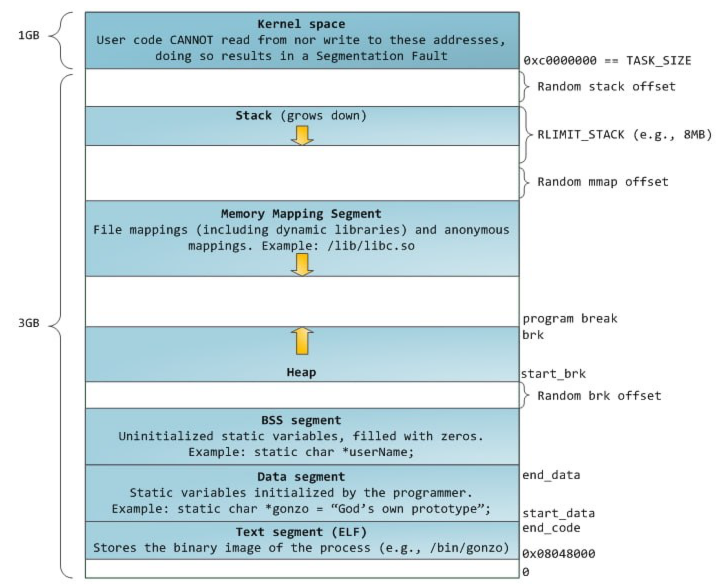
\includegraphics[width=15cm, ]{mem.png}
    \caption{Структура виртуальной памяти процесса из презентации}
\end{figure}
\newpage
\textbf{Кратко:}
\begin{itemize}
  \item data (статическая память). В этой секции лежат статические и глобальные переменные, а так же некоторые константы
\item text. В этом секции лежит машинный код
  \item stack (автоматическая память). Тут лежат локальные переменные и адреса возвратов
\end{itemize}
\textbf{Переполнение стека}
\begin{enumerate}
  \item Когда мы создаем какую-либо локальную переменную она кладется на стек. При выходе из области видимости эта переменная удалится со стека (снимется)
  \item На стек кладется адрес возврата, когда мы заходим в какую-либо функцию (иначе непонятно куда возвращаться после return в функции)
  \item Stack overflow (переполнение стека) - ситуация, когда пытаемся на стеке занять больше памяти чем есть (достаточно глубокая рекурсия)
\end{enumerate}
Размер стэка обычно ограничен 4мя или 8ю мегабайтами памяти
\subsubsection{Статические переменные}
Статические переменные:
Такую переменную можно завести не только внутри функции:
\begin{lstlisting}[language=C++]
int foo() {
  static int x = 0;
}
\end{lstlisting}
\textbf{Особенность:} переменная x будет проинициализирована только один раз, при первом вызове функции foo. И будет жить до конца программы, так что при каждом новом вызове функции foo мы будем работать с одной и той же переменной x.
\subsubsection{Операторы new/delete}
\begin{definition}{Динамическая память}{}
\textbf{Динамическая память} --- оперативная память из которой мы можем запрашивать кусочки. Эта память так же называется куча.
\end{definition}
\textbf{Оператор new}
Для выделения динамической памяти в плюсах служит оператор new. Его синтаксис: T* p = new T(...);
Выделим памяти на один int:
int* a = new int;

Теперь у нас есть 4 байта на куче. Можно было сразу проинициализировать на 10 элементов:
int* a = new int(10);
\newline
\textbf{Оператор delete}
Память, выделнную с помощью оператора new нужно "очищать". Для этого нужен оператор delete:
\begin{lstlisting}[language=C++]
int* a = new int(10);
delete a;
\end{lstlisting}
\textbf{Замечание: }после завершения программы вся память и так очистится, но вы много раз будете сталкиваться с ситуацией, когда память нужно очищать прямо во время работы программы

\subsubsection{Проблемы с памятью: memory leak и double free}
\begin{definition}{Memory leak}{}
\textbf{Memory leak} --- не убрали память за собой, потеряли указатель на нее, потом так вышло что программа вроде закончила работу, а пямять все еще за ней числится.
\end{definition}
\begin{definition}
{Double free}{}
\textbf{Double free} --- почистили 1 раз, а потом снова попытались, а там уже не наша память, RE
\end{definition}
\subsubsection{Массивы и операции над ними}
Для выделения массива служит другая версия оператора new: new int[size].
\begin{lstlisting}[language=C++]
int* arr = new int[10]; // Выделили массив из 10ти int
sizeof(arr); //  4 байта / 8  байт sizeof(int)
\end{lstlisting}
Указатель arr указывает на первый int в нашем массиве из 10ти интов и мы можем удобно работать с этой памятью:
\begin{lstlisting}[language=C++]
  for (int i = 0; i < 10; ++i) {
    arr[i] = i + 1;
  }
\end{lstlisting}
\textbf{Очистка}
\begin{lstlisting}[language=C++]
  delete[] arr;
\end{lstlisting}
\textbf{Важно:} Очищать память с помощью delete[] которая была выделена не с помощью new[] нельзя. Очищать память с помощью delete которая была выделена с помощью new[] тоже нельзя.
\textbf{СИшные массивы}
\begin{lstlisting}[language=C++]
  int arr[10]; // Массив из 10ти int на стеке
  for (int i = 0; i < 10; ++i) {
    arr[i] = i + 1;
  }
  sizeof(arr) // 40 байт (если int это 4 байта)
  int arr1[10];
  int arr2[10];
  arr1 = arr2; // CE
\end{lstlisting}
\newpage
\subsection{Вопрос 3}
\subsubsection{Базовый синтаксис функций}
\begin{definition}{Функция}{}
\textbf{Функция} --- блок кода, который выполняет какую-то операцию. Характеризуется четырьмя вещами: типом возвращаемого значения, названием, типами принимаемых аргументов (и их названиями) и телом.
\end{definition}
Объявление функции выглядит так:
\begin{lstlisting}[language=C++]
return_type function_name(ArgType1 arg1, ArgType2 arg2);

// например
int foo(int a, double b);
\end{lstlisting}
А определение --- это объявление плюс тело:
\begin{lstlisting}[language=C++]
return_type function_name(ArgType1 arg1, ArgType2 arg2) {
    your_code;
}
\end{lstlisting}
\textbf{Про return:} если возвращаемый тип не \texttt{void}, внутри функции обязан быть \texttt{return} с значением. Если \texttt{void}, то \texttt{return} тоже можно писать, но без аргумента --- удобно для досрочного выхода:
\begin{lstlisting}[language=C++]
void DevideAndPrint(int a, int b) {
    if (b == 0) {
        std::cout << "Devision by zero!";
        return;
    }
    std::cout << a / b;
}
\end{lstlisting}
\textbf{Важно:} аргументы в C++ передаются по умолчанию \textbf{по значению}, то есть копируются. Поэтому, например, классический \texttt{swap(a, b)} через \texttt{int}-аргументы работать не будет --- внутри функции мы поменяем местами копии, а снаружи ничего не изменится. Чтобы это починить, нужны указатели или ссылки (см. Вопрос 4).
\subsubsection{Аргументы по умолчанию}
\begin{definition}{Аргумент по умолчанию}{}
Значение, которое подставляется в параметр функции, если при вызове он не был передан явно.
\end{definition}
\begin{implementation}{Пример}{}
\begin{lstlisting}[language=C++]
int PlusWithLogging(int a, int b, bool logging = false) {
    if (logging) {
        std::cout << "Plus";
    }
    return a + b;
}

int main() {
    PlusWithLogging(1, 2);        // logging = false
    PlusWithLogging(1, 2, false);
    PlusWithLogging(1, 2, true);
}
\end{lstlisting}
\end{implementation}
\textbf{Правила:}
\begin{itemize}
  \item Сначала идут обычные аргументы (без значения по умолчанию), а уже потом --- все со значением по умолчанию. Перемешивать нельзя.
  \item Значение по умолчанию можно указать только один раз во всей программе (оно считается частью определения), иначе CE:
\begin{lstlisting}[language=C++]
void foo(int b = 10);
void foo(int b = 10) { return; } // CE: redefinition of default argument
\end{lstlisting}
\end{itemize}
\subsubsection{Перегрузка функций: простые примеры}
\begin{definition}{Перегрузка функций}{}
\textbf{Перегрузка} --- возможность иметь несколько функций с одинаковым именем, но разными списками аргументов. Компилятор сам выбирает нужную версию по типам переданных аргументов.
\end{definition}
\begin{implementation}{Пример}{}
\begin{lstlisting}[language=C++]
void foo(double) { std::cout << 1; }
void foo(int) { std::cout << 2; }

int main() {
    foo(10);  // выведет 2
    foo(5.0); // выведет 1
}
\end{lstlisting}
\end{implementation}
\textbf{Важно:} перегружать можно только по принимаемым аргументам. Две функции, отличающиеся лишь типом возвращаемого значения --- это не перегрузка, а CE:
\begin{lstlisting}[language=C++]
int foo(int a);
double foo(int a); // CE: foo cannot be overloaded
\end{lstlisting}
При этом возвращаемый тип у перегрузок может отличаться, если списки аргументов всё-таки разные:
\begin{lstlisting}[language=C++]
double plus(double, double);
double plus(int, int); // OK, аргументы разные
\end{lstlisting}
\subsubsection{Правила выбора перегрузки (базовое понимание)}
Полные правила выбора перегрузки можно посмотреть на \href{https://en.cppreference.com/w/cpp/language/overload_resolution}{cppreference}. Кратко (на базовом уровне):
\begin{enumerate}
  \item Если есть точное совпадение типов --- побеждает оно.
  \item Если точного совпадения нет, смотрят на \term{promotion} (например, \texttt{int} $\to$ \texttt{long}, \texttt{float} $\to$ \texttt{double}).
  \item Если и promotion нет, идут стандартные \term{conversion} (например, \texttt{int} $\to$ \texttt{double}).
\end{enumerate}
Если по этим правилам нельзя однозначно выбрать одну перегрузку (несколько одинаково подходят) --- получаем CE (\texttt{ambiguous call}):
\begin{lstlisting}[language=C++]
void foo(float) {}
void foo(int) {}

int main() {
    foo(5.0); // CE: call to foo is ambiguous
}
\end{lstlisting}
\textbf{Замечание:} \texttt{double -> float} и \texttt{double -> int} --- оба стандартных преобразования, и с точки зрения компилятора они равнозначны, поэтому выбрать одну версию нельзя.
\newpage
\subsection{Вопрос 4}
\subsubsection{Ссылки}
\begin{definition}{Ссылка}{}
\textbf{Ссылка} --- это, по сути, второе имя (псевдоним) уже существующей переменной. Объявляется добавлением \texttt{\&} к типу: \texttt{T\& name = obj;}. Концепции ссылок в языке C нет, это фича C++.
\end{definition}
\begin{implementation}{Пример}{}
\begin{lstlisting}[language=C++]
int a = 1;
int& b = a; // b -- это теперь тоже имя переменной a

b = 5;
std::cout << a; // 5, потому что a и b -- одна и та же переменная
\end{lstlisting}
\end{implementation}
\textbf{Зачем нужны:}
\begin{itemize}
  \item Создавать псевдонимы для переменных.
  \item Легковесно передавать аргументы в функции без копирования и без возни с разыменованием указателей. Если бы мы передавали \texttt{std::vector<int>} по значению, при каждом вызове он бы целиком копировался.
\end{itemize}
\textbf{Важные свойства ссылок:}
\begin{itemize}
  \item Ссылку \textbf{нельзя} объявить без инициализации --- ей сразу нужно к чему-то привязаться.
  \item Ссылку можно проинициализировать только lvalue (то есть нельзя написать \texttt{int\& a = 10;}).
  \item Ссылка привязывается к объекту \textbf{один раз и навсегда} --- перепривязать её к другому объекту нельзя (\texttt{ref = other;} просто присвоит \texttt{other} в объект, на который указывает \texttt{ref}, а не перепривяжет ссылку).
  \item На текущем уровне знаний ссылку нельзя никак отличить от переменной, на которую она ссылается (даже адрес совпадает).
  \item Нельзя перегружать функции по признаку "ссылка/не ссылка" на один и тот же тип:
\begin{lstlisting}[language=C++]
void f(int& c) {}
void f(int c) {}
int main() {
    int a;
    f(a); // CE: ambiguous, перегрузки неразличимы
}
\end{lstlisting}
  \item Нельзя: указатель на ссылку (\texttt{int\&* a;} --- CE), массив ссылок, ссылку на ссылку.
\end{itemize}
\textbf{Возврат ссылок из функций:} можно вернуть ссылку на объект, который продолжит жить после выхода из функции (например, на переданный по ссылке аргумент):
\begin{lstlisting}[language=C++]
int& f(int& x) {
    ++x;
    return x;
}
int main() {
    int a = 10;
    f(a) = 20; // OK, f(a) -- это lvalue (ссылка на a)
}
\end{lstlisting}
А вот вернуть ссылку на локальную переменную --- UB (висячая ссылка, dangling reference), потому что объект уничтожается при выходе из функции:
\begin{lstlisting}[language=C++]
int& f() {
    int x = 10;
    return x; // UB
}
int main() {
    int& a = f();
    a = 10; // UB: обращаемся к уже разрушенному объекту
}
\end{lstlisting}
\textbf{Замечание:} уничтожение самой ссылки (выход из её области видимости) не уничтожает объект, на который она ссылается:
\begin{lstlisting}[language=C++]
int main() {
    int a = 10;
    {
        int& b = a;
    } // b умерла, a жива
    a = 5; // OK
}
\end{lstlisting}
\subsubsection{Константы}
\begin{definition}{const}{}
\textbf{const T} --- это тип, который ведёт себя почти так же как \texttt{T}, но поддерживает меньше операций: объект, объявленный как \texttt{const}, нельзя изменять.
\end{definition}
\begin{implementation}{Пример}{}
\begin{lstlisting}[language=C++]
int main() {
    const int a = 5;
    // a = 6; -- CE
}
\end{lstlisting}
\end{implementation}
\textbf{4 способа передать аргумент в функцию:}
\begin{itemize}
  \item По значению (будет копия).
  \item По константному значению (бессмысленно для базового использования, так почти не пишут).
  \item По ссылке (можем менять исходный объект, копии нет).
  \item По константной ссылке (без копии, но изменить объект через эту ссылку нельзя).
\end{itemize}
\textbf{Замечание:} можно перегружать функции по константной/неконстантной ссылке.
\textbf{Продление жизни:} константной ссылке можно присвоить временный объект --- время жизни этого временного объекта продлевается до времени жизни ссылки:
\begin{lstlisting}[language=C++]
int main() {
    const int& a = 5; // временный объект 5 проживёт столько же, сколько a
}
\end{lstlisting}
\subsubsection{Навешивание констант на указатели и ссылки}
Константу можно "навесить" на уже знакомые нам указатели несколькими способами.
\textbf{Указатель на константу} (менять можно сам указатель, но не то что под ним):
\begin{lstlisting}[language=C++]
int a;
const int* ptr = &a;
\end{lstlisting}
\textbf{Константный указатель} (менять нельзя сам указатель, но можно то, что под ним):
\begin{lstlisting}[language=C++]
int a;
int* const ptr = &a;
\end{lstlisting}
\textbf{Константный указатель на константу} (нельзя менять ни то, ни другое):
\begin{lstlisting}[language=C++]
int a;
const int* const ptr = &a;
\end{lstlisting}
\begin{implementation}{Все случаи сразу}{}
\begin{lstlisting}[language=C++]
int main() {
    int a = 5;

    const int* p = &a;
    ++p;   // OK, сам указатель не const
    ++*p;  // CE, то, на что указывает p, -- const

    int* const pp = &a;
    ++pp;  // CE, указатель pp -- const
    ++*pp; // OK

    const int* const ppp = pp; // OK: cast от int* к const int* разрешен
    ++ppp;  // CE
    ++*ppp; // CE

    int* const q = ppp; // CE, запрещённый каст (теряем константность)
    const int* qq = ppp; // OK, просто копия
}
\end{lstlisting}
\end{implementation}
Аналогично можно навесить константу на ссылку --- константная ссылка даёт доступ только на чтение, и присвоить её обычной (неконстантной) ссылке нельзя:
\begin{lstlisting}[language=C++]
int main() {
    int a = 5;
    const int& ref = a;
    int& b = ref; // CE: теряем константность
}
\end{lstlisting}
\newpage
\subsection{Вопрос 5}
\subsubsection{Абстракция, инкапсуляция, наследование, полиморфизм}
\begin{definition}{Абстракция}{}
\textbf{Абстракция} --- выделение значимой информации об объекте и исключение из рассмотрения незначимой. В ООП обычно говорят про абстракцию данных: набор наиболее важных характеристик объекта, доступных остальной программе.
\end{definition}
\begin{definition}{Инкапсуляция}{}
\textbf{Инкапсуляция} --- свойство системы, позволяющее объединить данные и методы, которые с этими данными работают, в одной сущности (классе).
\end{definition}
\textbf{Замечание:} в C++ под инкапсуляцией часто понимают ещё и сокрытие данных (через \texttt{private}), но вообще говоря это необязательное условие самой инкапсуляции.
\begin{definition}{Наследование}{}
\textbf{Наследование} --- свойство системы, позволяющее описать новый класс на основе уже существующего, частично или полностью заимствуя его функциональность.
\end{definition}
\begin{definition}{Полиморфизм}{}
\textbf{Полиморфизм} (точнее, полиморфизм подтипов) --- свойство системы, позволяющее использовать объекты с одинаковым интерфейсом, не зная их точного типа и внутреннего устройства.
\end{definition}
\subsubsection{Классы, объекты, члены классов, поля, методы}
\begin{definition}{Класс}{}
\textbf{Класс} --- кастомный (придуманный программистом) тип данных, состоящий из набора \term{полей} и \term{методов} для взаимодействия с ними.
\end{definition}
\textbf{Замечание:} до некоторого момента \texttt{class} и \texttt{struct} в C++ --- абсолютно одно и то же (разница только в модификаторе доступа по умолчанию, см. Вопрос 1 секции "на уд").
\begin{lstlisting}[language=C++]
class MyAwesomeClass {
    // ...
};

int main() {
    MyAwesomeClass c; // c -- объект (он же экземпляр) класса MyAwesomeClass
    sizeof(c); // 1, у пустого класса есть минимальный ненулевой размер
}
\end{lstlisting}
\textbf{Поля} --- это данные, которые хранит в себе объект. \textbf{Методы} --- это функции, которые можно совершать над объектом данного класса (внутри методов нам доступны поля объекта, для которого метод вызван).
\begin{implementation}{Структура с полями и методом}{}
\begin{lstlisting}[language=C++]
struct Student {
    std::string name;
    size_t grade;

    void Print() {
        std::cout << name << " " << grade << std::endl;
    }
};
\end{lstlisting}
\end{implementation}
\textbf{Важно:} если не задать полям значения по умолчанию, то при объявлении объекта без явной инициализации в полях окажется мусор (для встроенных типов) либо значение по умолчанию для типа поля (например, пустая строка для \texttt{std::string}):
\begin{lstlisting}[language=C++]
struct Student {
    std::string name = "Test"; // теперь по умолчанию не мусор
    size_t grade = 10;
};
\end{lstlisting}
Методы можно объявлять внутри класса, а определять --- снаружи, через оператор \texttt{::}:
\begin{lstlisting}[language=C++]
struct Student {
    std::string name;
    size_t grade;

    void Print(); // объявили
};

void Student::Print() { // определили
    std::cout << name << " " << grade << std::endl;
}
\end{lstlisting}
\subsubsection{Операторы . , -> , ключевое слово this}
\begin{itemize}
  \item Оператор \texttt{.} --- обращение к полям и методам объекта.
  \item Оператор \texttt{->} --- обращение к полям и методам через указатель на объект (синтаксический сахар для \texttt{(*ptr).field}).
\end{itemize}
\begin{lstlisting}[language=C++]
int main() {
    Student student;
    student.Print();   // через объект

    Student* ptr = &student;
    ptr->Print();       // через указатель
}
\end{lstlisting}
\begin{definition}{this}{}
Внутри любого нестатического метода класса неявно определён указатель \texttt{this} --- указатель на тот объект, для которого метод был вызван.
\end{definition}
\begin{implementation}{Зачем нужен this}{}
\begin{lstlisting}[language=C++]
struct Student {
    std::string name = "Test";

    void SetName(std::string name) {
        this->name = name; // отличаем поле от параметра с тем же именем
    }
};
\end{lstlisting}
\end{implementation}
\newpage
\subsection{Вопрос 6}
\subsubsection{Перечисления (enum): примеры и как с ними работать}
\begin{definition}{enum}{}
\textbf{Перечисление (enum)} --- способ объявить свой тип как набор именованных констант.
\end{definition}
\begin{implementation}{Обычный enum}{}
\begin{lstlisting}[language=C++]
enum Color {
    RED,
    GREEN,
    BLUE,
    YELLOW
};

Color c = BLUE; // так писать не стоит, см. ниже
\end{lstlisting}
\end{implementation}
\textbf{Проблема:} обычный \texttt{enum} вносит все свои константы (\texttt{RED}, \texttt{GREEN}, ...) в окружающую область видимости, что легко приводит к конфликту имён. Поэтому в C++11 ввели \texttt{enum class}:
\begin{implementation}{enum class}{}
\begin{lstlisting}[language=C++]
enum class Color {
    RED,
    GREEN,
    BLUE
};

Color c = Color::BLUE; // обращение через имя enum
\end{lstlisting}
\end{implementation}
По умолчанию константы нумеруются с 0 по порядку (\texttt{RED} = 0, \texttt{GREEN} = 1, \texttt{BLUE} = 2). Можно явно задавать числовые значения, а необозначенные продолжат счёт от последнего заданного:
\begin{lstlisting}[language=C++]
enum class Foo {
    a,         // 0
    b,         // 1
    c = 10,    // 10
    d,         // 11
    e = 1,     // 1 (можно повторять значения)
    f,         // 2
    g = f + c, // 12
};
\end{lstlisting}
Можно явно указать, константами какого целочисленного типа являются значения \texttt{enum} (по умолчанию это обычно \texttt{int}):
\begin{lstlisting}[language=C++]
enum class Color : int8_t {
    RED,
    GREEN,
    BLUE
};
\end{lstlisting}
